\documentclass[11pt]{article}% uses letterpaper by default

%---------- Uncomment one of them ------------------------------
\usepackage[includeheadfoot, top=0.5in, bottom=0.5in, hmargin=1in]{geometry}

% \usepackage[a5paper, landscape, twocolumn, twoside,
%    left=2cm, hmarginratio=2:1, includemp, marginparwidth=43pt,
%    bottom=1cm, foot=.7cm, includefoot, textheight=11cm, heightrounded,
%    columnsep=1cm, dvips,  verbose]{geometry}
%---------------------------------------------------------------
\usepackage{fancyhdr}
\usepackage{setspace}
\renewcommand{\footrulewidth}{0.4pt}% default is 0pt
\usepackage[makeroom]{cancel}
\pagestyle{fancy}
\usepackage{graphicx}
\singlespacing
\usepackage{amsmath}

\newcommand{\degrees}{\ensuremath{^\circ}}
\newcommand{\arcmin}{\ensuremath{'}}
\newcommand{\arcsec}{\ensuremath{"}}
\newcommand{\hours}{\ensuremath{^\mathrm{h}}}
\newcommand{\minutes}{\ensuremath{^\mathrm{m}}}
\newcommand{\seconds}{\ensuremath{^\mathrm{s}}}

%\newcommand{\s}[0]{\phantom{i}} %sets up \s command
%\newcommand{\m}[0]{\phantom{abcde}} %sets up \m command
\providecommand{\e}[1]{\ensuremath{\times 10^{#1}}} %sets up \e command
%\setlength{\parindent}{0.2in} %new paragraph indent
%\usepackage{indentfirst} % indent the first paragraph of a section

\newcommand{\labnumber}{01}  % UPDATE THIS!

\usepackage{hyperref}
\hypersetup{
	colorlinks = true,
	urlcolor = cyan,  % Links to URLs
	linkcolor = cyan  % Links within PDF
}

\usepackage{etoolbox}
\newtoggle{teacher}
\toggletrue{teacher}  % Set TRUE to print instructor notes
%\togglefalse{teacher}  % Set FALSE to hide instructor notes
% This doesn't work for multiple paragraphs
\newcommand*{\annote}[1]{\textcolor{blue}{\textbf{Instructor notes:} {#1}}}

\usepackage{enumitem}  % modifies enumerate, itemize
%\setlist{noitemsep}
\usepackage{multicol}

% Compact spacing
\setlength\parindent{0pt}
\setlength{\parskip}{1em}

\newcommand*{\mt}{\mathrm}
\newcommand*{\unit}[1]{\;\mathrm{#1}}  % vemod.net/typesetting-units-in-latex
\newcommand*{\Msun}{\mathrm{M}_{\sun}}

\usepackage{datetime2}  % customize \today, defaults to yyyy-mm-dd
\lhead{ASTR UN1903 -- Lab \labnumber}
\lfoot{M. Sayeed}
\cfoot{\thepage}
\rfoot{\today}
\rhead{Mondays 6-9 pm}
\renewcommand{\rightmark}{}
\renewcommand{\headrulewidth}{0pt}
\renewcommand{\footrulewidth}{0.4pt}
% -----------------------------
% End personal config (AT, Sp 2019)
% -----------------------------

\begin{document}

\begin{center}
    \LARGE Lab \labnumber: Units and Orders of Magnitude
\end{center}

\iftoggle{teacher}{
Astronomy asks us to ponder structures and systems on scales way outside the realm of human experience.  From itty-bitty atoms to massive clusters of galaxies, from the speed of light to the age of stars, the sheer extremity of the numbers we toss around sometimes allows them to lose their meaning.  If I tell you that Jupiter has a mass of 1,898,000,000,000,000,000,000,000,000 kg, it probably won't mean much to you.  However, a working understanding of numbers, units, and especially \textit{orders of magnitude} is a vital tool of scientific literacy.  The skills we will develop today allow us to rescue numbers from mathematical abstraction and root them in a familiar context.}{}

\section{A Review on Numbers and Units}

Please answer in your lab notebooks, showing all work.
No calculators, electronics, or asking your neighbor (just for now).
% \textbf{This quiz will be graded for completion, not correctness.}

\begin{enumerate}[label=\textbf{\alph*.}]
    %\renewcommand{\theenumi}{\alph{enumi}}  % if not using enumitem
    %\renewcommand{\labelenumi}{(\alph{enumi})}
    \item Write down the metric (or Syst\`{e}me International, SI) prefixes and
        abbreviations for:
        \[
            %10^{-12} \quad\quad
            10^{-9} \quad\quad
            10^{-6} \quad\quad
            10^{-3} \quad\quad
            10^{0} \quad\quad
            10^{3} \quad\quad
            10^{6} \quad\quad
            10^{9}
        \]

    \item Sketch a graph and plot the following data points:
        \[
            (  1.1, 300) \quad
            ( 11,   120) \quad
            (100,    30) \quad
            (900,    10)
        \]

    \item What is
        $\left(3 \times 10^{14} \unit {m} \right) \times \left(3 \times
        10^{-8}\right) / \left(4.5 \times 10^{11}\right)$ ?
        Write your answer in scientific notation.  Which SI prefix from above
        is closest to this value?

    \item Astronomers (including you, now!) often use funny units because we
        must study phenomena on a wide range of scales.
        A Megaparsec (Mpc) is about the distance to the Andromeda Galaxy.
        A cubic Megaparsec is thus a good unit for, say, finding the density of
        galaxies in the universe.

        What is $1 \unit{Mpc^3}$ in $\mt{m^3}$?
        Note that $1 \unit{parsec} = 3.1 \times 10^{16} \unit{m}$.

    \item A radio message is broadcast to Voyager 2, which is
        $2.2 \times 10^{13} \unit{m}$ from Earth (as of 2019 Jan 29).
        Radio waves travel at the speed of light,
        $c = 3.0 \times 10^{8} \unit{m/s}$.
        How many hours will it take for the message to reach Voyager?
        % expected answer: 20:07:06 hh:mm:ss
\end{enumerate}

% At the start of next lab, we'll have another short quiz extremely similar to this, but graded for correctness.

\iftoggle{teacher}{
}{
\newpage
\pagebreak
}

\section{Units and Equations}

\begin{center}
    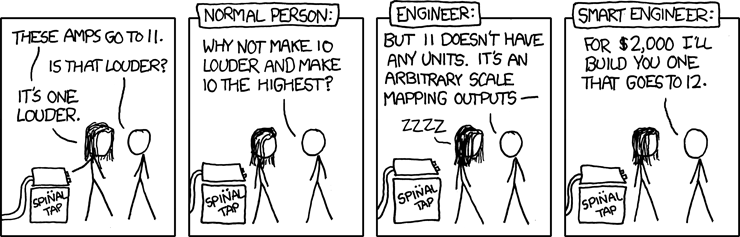
\includegraphics[width=\textwidth]{xkcd_670.png} \\
    Source: \href{https://xkcd.com/670/}{xkcd.com/670}
\end{center}

Centimeters, miles, kilograms, and years are examples of \textit{units}.
Every number we will deal with in this lab represents \emph{something}, and
almost all such numbers will require a unit.
Class is not 3 long -- it is 3 \emph{hours} long.
The Brooklyn Bridge is not 1.13 across -- it is 1.3 \emph{miles} across.
For dinner, you did not eat 2 -- you ate 2 \emph{apples}.
Whenever you report a measurement, you must include the unit.

\subsection{Converting Units}

Your units must agree in all calculations.
You can't add centimeters and meters until you convert them to the same units.
You can't say $X = Y$ if $X$ is in kilograms and $Y$ is in seconds.

To convert units, multiply by a fraction that's equal to 1:
$\frac{1 \,\mathrm{year}}{365 \,\mathrm{days}}$,
$\frac{12 \,\mathrm{inches}}{1 \,\mathrm{foot}}$,
etc.

For example, to convert 1 year to seconds:
\begin{flalign*} % https://tex.stackexchange.com/a/28664
    &\quad 1 \unit{year}&
\end{flalign*}

Or, to convert 5 acres to $\unit{m^2}$
($1 \unit{acre} = 66 \unit{ft} \times 660 \unit{ft}$,
and $1 \unit{ft} = 0.3048 \unit{m}$):
\begin{flalign*}
    &\quad 5 \unit{acre}&
\end{flalign*}
As a general rule, you can treat units like multiplicative constants.

% \iftoggle{teacher}{{do examples on the board.  Tell students some or all of: ``It may take several steps to reach the unit you want. You should explicitly write out your unit conversion as above. This is good practice, and I recommend that you always do this; keeping track of units will prevent mistakes and keep you sane!''}}{}

Convert the following, showing your conversion steps explicitly.
Note $1 \unit{mi} = 1.609 \unit{km}$.
\begin{itemize}
\item Typical human height: 5'9'' (5 feet and 9 inches) $\to$ meters
%\item \textbf{Distance from the Earth to the Sun (1 AU)} %1.5*10^11 m, or 10^11 m
\item One marathon: 26.2 miles $\to$ kilometers
\item A speed limit: 65 miles per hour $\to$ kilometers per second
\end{itemize}

\subsection{Simplifying Units}

Many quantities have units that are some combination of mass, length, and time,
multiplied or divided together.  For example, acceleration has units
$\mathrm{m/s^{2}}$, length over time squared.
One convention is to write the units of a quantity like so:
\[
    \left[ a \right] = \mt{\left[ \frac{m}{s^2} \right]}
\]
%Angles (degrees/radians) and temperatures (Kelvin) are special: these are
%called \emph{dimensionless}, but we attach rad, $^{\circ}$, K to help ourselves
%keep track of what the numbers mean.
%In practice, we often treat these like units anyways.
Write down the units of each quantity below using only meters, kilograms, and
seconds (MKS units).
The right-side variables are $m =$ mass, $a =$ acceleration,
$c =$ speed of light, $t =$ time, and $r =$ distance.
%and $G = 6.67 \times 10^{-11} \unit{m^3/s^2/kg}$ (Newton's gravitational constant).

\begin{itemize}%[itemsep=2pt]
    \item Force: $F = m a$
        %\hfill\soln{$\mathrm{ kg \; m \; s^{-2} }$}
    \item Energy: $E = m c^2$
        %\hfill\soln{$\mathrm{ kg \; (m/s)^2 = kg \; m^2 \; s^{-2} }$}
    \item Power: $L = E / t$
        %\hfill\soln{$\mathrm{ kg \; m^2 \; s^{-3} }$}
    \item Flux: $F = L / (4 \pi r^2)$
        %\hfill\soln{$\mathrm{ kg \; s^{-3} }$}
    %\item ????: $P = 2 \pi d^{3/2} / (G m)^{1/2}$
        %\hfill\soln{$\mathrm{ m^{3/2} / (m^3/s^2/kg \times kg)^{1/2}
        %                      = m^{3/2} / (m^{3/2} / s)
        %                      = s }$}
\end{itemize}

Some quantities have units that can't be reduced to just meters, kilograms, and
seconds.
\begin{itemize}
    \item Can you think of some examples?  Give at least two.
    \item Can you think of, or make up, a quantity that has no units?
        Such a quantity is called \emph{unitless} or \emph{dimensionless}.
        Think of and define one such quantity, and write it down.
\end{itemize}

% \iftoggle{teacher}{\annote{
%     If your dinner is 2 apples, you can say that the unit of food is an
%     ``apple''.  This can't be written in terms of mass, length, and time, but
%     you can treat it like any other unit.  If you eat 2 apples per day, you can
%     compute how many apples you eat per year.
% }}{
% }

\iftoggle{teacher}{{One type of value that won't have units is a ratio of like units: if someone is twice as old as you, we say they are ``two times'' older, and that two is ``unitless''. This is because if your age is 20 years and your friend's age is 40 years, the ratio of your ages is $\frac{40 \,\mathrm{years}}{20 \,\mathrm{years}}$ = 2: the units cancel.}}{
}

\subsection{Detective Work with Units}

\begin{center}
    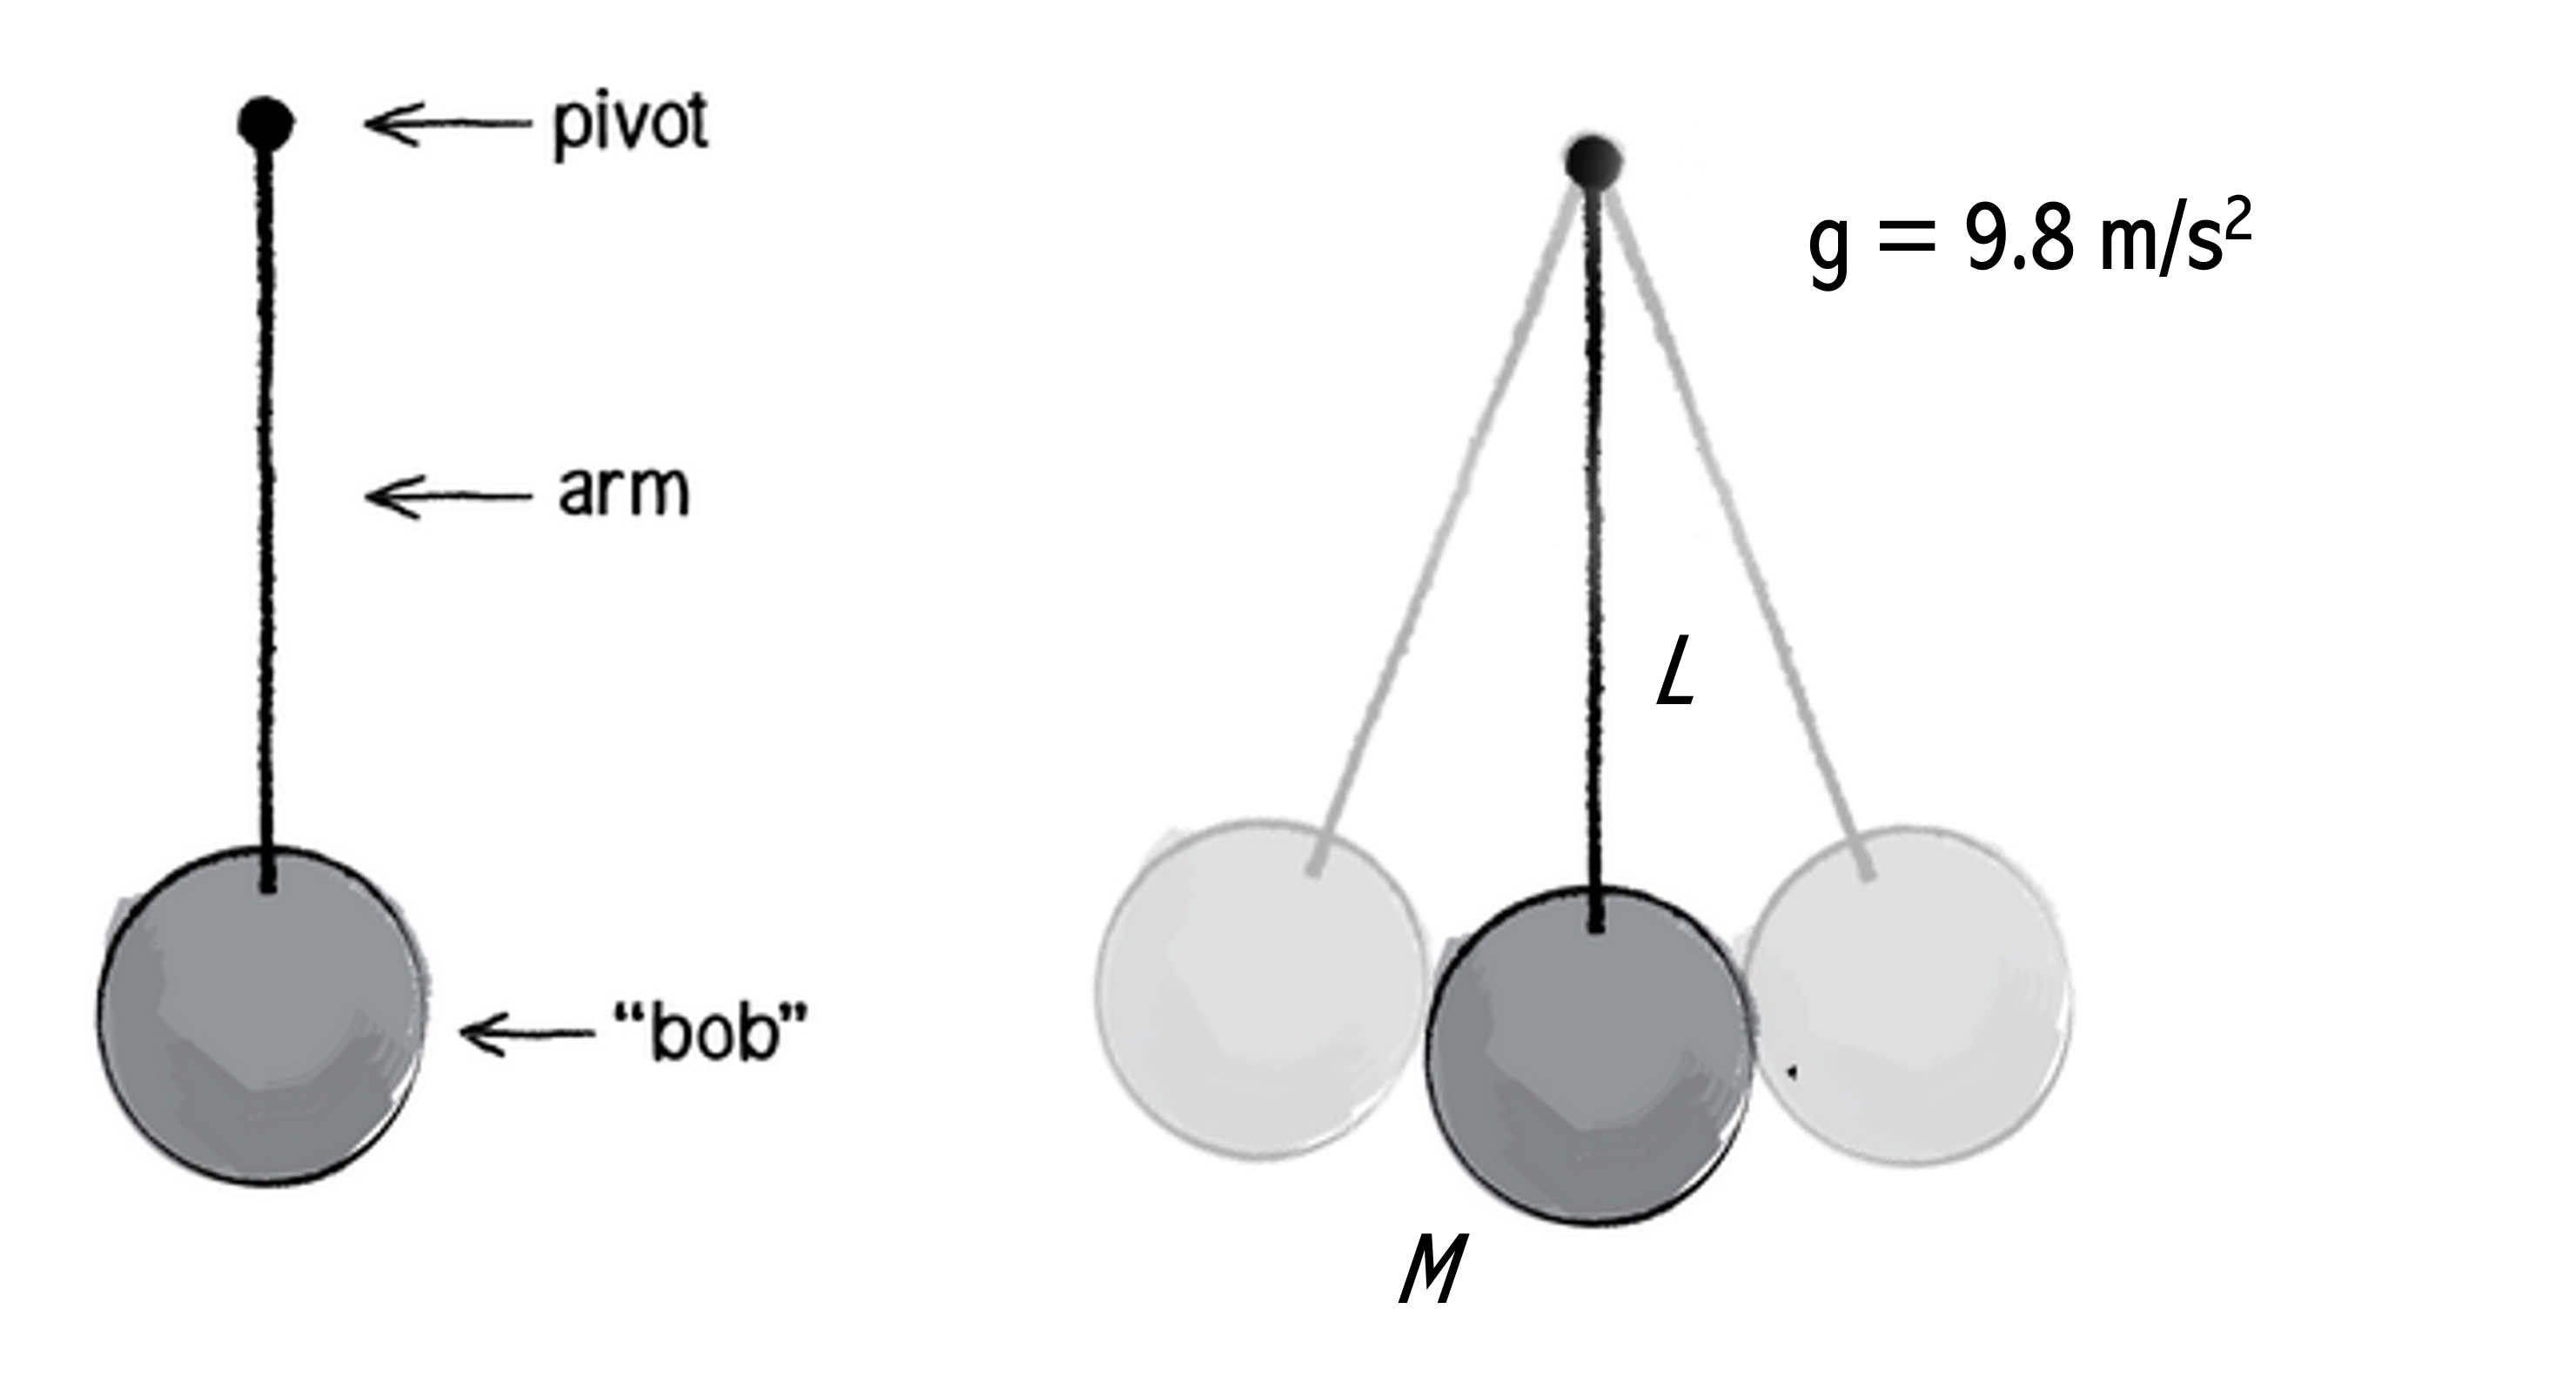
\includegraphics[width=0.5\textwidth]{pendulum.png}
\end{center}

Consider a pendulum of length $L$ and mass $M$ swinging in the Earth's
surface gravitational field.
The period $T$ between successive swings can depend only on $M$, $L$, $g$.
%I.e., $T$ is an unknown function $T(M, L, g)$.
Which of the below options is the correct equation for pendulum's period? Explain. Hint: $L$ is usually measured in metres ($m$) and $M$ is usually measured in kilograms ($kg$). \textit{Do not look up the formula online!}

\begin{align*}
\begin{aligned}[c]
T &= 2 g M / L \\
T &= 2\pi L^2 / (M g) \\
T &= 2 M \sqrt{g} \\
T &= g \sqrt{L} \\
T &= 2\pi \sqrt{L / g}
\end{aligned}
\qquad\qquad
\qquad\qquad
\begin{aligned}[c]
T &= 2 \pi g M / L \\
T &= \pi g M^2 / L^3 \\
T &= \sqrt{2 M g} \\
T &= 2\pi L / M \\
T &= 2\pi \sqrt{g / L}
\end{aligned}
\end{align*}

%\begin{enumerate}[label=\textbf{\alph*.}]
%    %\renewcommand{\theenumi}{\alph{enumi}}
%    \item $T = 2 g L / M$
%    \item $T = 2 g L / M$
%    \item $T = g \sqrt{L}$
%    \item $T = \frac{\pi L^2}{g}$
%    \item $T = 2\pi \sqrt{\frac{g}{L}}$
%    \item $T = 2\pi \sqrt{\frac{L}{g}}$
%\end{enumerate}

\iftoggle{teacher}{
}{
\newpage
\pagebreak
}

Suppose you are taking an exam in Prof. Appelgate's Earth, Moon, and Planets class. On the provided formula sheet you see two equations:
\begin{align*}
    F &= \frac{G m_1 m_2}{r^2} \\
    P &= \frac{ 2 \pi r^{3/2} }{ \left( G m \right)^{1/2} }
\end{align*}
Pretend: you don't remember what these equations mean, but you do
recall the following facts:
\begin{itemize}
    \item $F$ is a force
    \item $r$ is a distance between two unspecified objects
    \item $m_1$, $m_2$, and $m$ are masses of some unspecified objects
    \item $G$ is Newton's gravitational constant, but you don't remember its value or units
\end{itemize}

What are the units of $P$ and $G$? 
% To help yourself guess at what $P$ means, figure out -- \textbf{what are the units of $P$}?

\section{Orders of Magnitude}

%\center
%\includegraphics{xkcdoom.png} \\
%\emph{credit: what-if.xkcd.com}
\begin{center}
    
\includegraphics[width=0.5\textwidth]{xkcd_oom.png} \\
    Source: \href{https://what-if.xkcd.com/84/}{what-if.xkcd.com/84}
\end{center}

The \emph{order of magnitude} of a value is the ``power of ten'' that is
closest to that value.
To find the order of magnitude, write your value in scientific notation
$m \times 10^n$ and round the coefficient $m$ to either 1 or 10.
You should end up with $10^x$, where $x$ is a positive or negative integer.
For instance, $0.001$, $1$, and $1,000,000$ are orders of magnitude, though
they are usually written in exponential form: $10^{-3}$, $10^0$, and $10^6$.

%To write a number in scientifc notation, find the first non-zero digit in the highest place (the left-most place; in this case it's the 6), and put the decimal point after that digit.  Then count how many places you move the decimal place, which gives you the power of ten (in this case it's 8; convince yourself that this is true).  If you move the decimal place left, the power of ten is positive.  If you have to move the decimal place to the right (i.e. the number is less than 1), then the power of ten is negative.  We can then say that the Sun's radius is $6.95\times10^8$.

Scientists use orders of magnitude when knowing the specific value of a number
is not necessary or practical.
If you want to compare the radii of the Sun and Earth, it often suffices to
know if the Sun's radius is $0.01\times$, $100\times$, or $1,000,000\times$ the
Earth's radius.

In this course, you will calculate many numbers.
You should regularly ask yourself, ``Is my order of magnitude reasonable?''
For example, if you measure the height of Pupin Hall to be of order $10
\unit{cm}$, you'd immediately know that your answer is wrong.

%pre-calculation step is to estimate what order of magnitude your value should
%be.
%If I asked you to calculate the height of Pupin and you got an answer on the
%order of 10 cm, you would immediately know that value was wrong.
%Similarly, if you calculated the speed of a rocket to be 400,000 km/s, you
%can immediately know that your speed is incorrect (why is it incorrect?).

\textbf{Describe what an order of magnitude is, in your own words}.
Then determine the order of magnitude for the following quantities:
\begin{itemize}
    \setlength\itemsep{0.2em}
    \setlength\parskip{0em}
    \item 123456789.
    \item 0.00000768
    \item 994.
    \item 50 seconds.
    \item 373 m (Empire State Building's 102nd floor observatory height) %10^2 m
\end{itemize}

% \iftoggle{teacher}{{
% Note that $\log_{10}(358) = 2.57$, so this is quite close to halfway between
% $10^2$ and $10^3$.
% }}{
% }

%One type of value that won't have units is a ratio of like units:
%if someone is twice as old as you, we say they are ``two times'' older, and
%that two is ``unitless''.
%This is because if your age is 20 years and your friend's age is 40 years, the ratio of your ages is $\frac{40 \,\mathrm{years}}{20 \,\mathrm{years}}$ = 2: the units cancel.

\subsection{Powers of Ten}

How good is your intuition for orders of magnitude?
Place the following items on a nice big number line spanning $10^{-16}$ to
$10^{24}$ meters.
\textit{Don't look anything up, though you may discuss with your peers! Give your best estimates.}

\begin{itemize}
\begin{multicols}{2}
\setlength\itemsep{0.2em}
\setlength\parskip{0em}
%\item Human hair thickness
\item Earth
\item 1 light-second
\item Proton
\item Distance to the nearest star
\item Milky Way
\item Red blood cell
\item Virgo Supercluster of galaxies
\item Ant
%\item 1 light-nanosecond
\item Sun
\item Distance to Andromeda
\item Human
\item Length of Lake Michigan
\item Distance to Pluto
\item DNA nucleotide
\item Moon
\item Distance the Sun
\end{multicols}
\end{itemize}

% Rough ordering
%\item Proton
%\item DNA nucleotide
%\item Red blood cell
%\item Human hair width
%\item Ant
%\item 1 light-nanosecond
%\item Human
%\item Length of Lake Michigan
%\item Hurricane
%\item Moon
%\item Earth
%\item Sun
%\item 1 light-second
%\item Distance to the Moon
%\item Distance to the nearest star (Proxima Centauri)
%\item Distance to Andromeda
%\item Milky Way
%\item Virgo Supercluster of galaxies

Then we'll watch a short movie called ``Powers of Ten'':
\href{https://youtu.be/0fKBhvDjuy0}{youtu.be/0fKBhvDjuy0} \\
and a spoof thereof:
\href{https://youtu.be/FEuEx1jnt0M}{youtu.be/FEuEx1jnt0M}

% \iftoggle{teacher}{\annote{Tell people to pay attention here -- mark up their second number line. Wolfram|Alpha gives (radius of Sun) / (radius of Earth) = 109.2.}}{}

\begin{itemize}
\item Compare your estimates to the actual sizes. How good were your estimates? For which objects was your intuition good, or not so good?
\item How many Earths can you line up along the diameter of the sun? Give an answer to order-of-magnitude precision (so, an answer within $3\times$ or $1/3\times$ the correct value is good).
\end{itemize}

\iftoggle{teacher}{
}{
\newpage
\pagebreak
}

% === SKIPPING THIS SECTION FOR FIRST LAB
% \section{Order of Magnitude Physics}

% %How many Earths would fit inside the Sun?
% How many cells do you have in your body?
% How long would it take you to walk to Delaware?
% If the universe was scaled so that the Sun was the size of a basketball, how
% far away would the nearest star be?
% Which is less dense, the solar system or an atom?
% How many piano tuners are there in Manhattan?
% You now have all the tools to answer these questions, and many more!

% \textbf{Choose one question, or make your own, and attempt to answer it.} Note: if time is short, we may skip this section of the lab and go to the conclusions.

% A few guidelines and potentially useful bits of information:
% \begin{itemize}
% \setlength\itemsep{0.2em}
% \setlength\parskip{0em}
% \item Try your best not to look up any numbers; if you think you need to look something up, try asking your peers or instructor for ideas before turning to
% Google. For this exercise, it is okay to ask for or look up formulas, e.g., volume of a sphere.
% \item When doing order-of-magnitude calculations, keep one significant figure.
% For example, if you have an intermediate calculation like:
% \[
%     27 \unit{miles/gallon} \times 150 \unit{gallon} = 4050 \unit{miles}
% \]
% you can report this as $4 \times 10^{3} \unit{miles}$, and use the
% lower-precision result for any subsequent calculations.
% \item Sun's mass: ${1.989 \e {30}} \unit{kg}$.
% \item Neptune's orbital radius: $30.10366151 \unit{AU}$; note
% $1 \unit{AU} = 1.496 \e {11} \unit{m}$.
% \item Hydrogen atom mass: ${1.66 \e {-24}} \unit{g}$.
% \end{itemize}

%Air has a density of $1.3 \, \mathrm{kg}/\mathrm{m}^3$.
%How does this compare to the two densities you just calculated?
%(How many orders of magnitude is it off by?)

\section{Conclusions}

\begin{enumerate}
    \item In general terms, when is the order-of-magnitude precision enough?
    When is it not?  Give some examples and explain.
    \item In the Simpsons spoof of ``Powers of Ten'', the universe was itself
    embedded within atoms of a greater universe.  Do you think our universe
    could be embedded in another universe in the same way?  If so, how could we
    tell?
    \item What did you like or dislike about this lab? Any suggestions? Leave comments in your lab notebook.
    \item What is one (or more!) remaining question(s) you have after completing this lab?
    
\end{enumerate}

Lastly, if you liked thinking about orders-of-magnitude, you may also enjoy
this visualization of what the solar system would look like if the Moon were 1
pixel wide:\\
\href{http://joshworth.com/dev/pixelspace/pixelspace_solarsystem.html}{joshworth.com/dev/pixelspace/pixelspace\_solarsystem.html}

\end{document}
